\documentclass[11pt,a4paper]{article}

\usepackage[utf8]{inputenc}
\usepackage[T1]{fontenc}
\usepackage{lmodern}
\usepackage[margin=2.3cm]{geometry}
\usepackage{booktabs}
\usepackage{tabularx}
\usepackage{array}
\usepackage{enumitem}
\usepackage[font=small]{caption}
\usepackage{url}
\usepackage[hidelinks]{hyperref}
\usepackage{tikz}
\usetikzlibrary{positioning,arrows.meta}

\renewcommand{\arraystretch}{1.15}
\newcolumntype{L}{>{\raggedright\arraybackslash}X}
\setlength{\parskip}{0.45em}
\setlength{\parindent}{0pt}
\setlist{itemsep=1pt,topsep=2pt}
\renewcommand{\topfraction}{0.9}
\renewcommand{\bottomfraction}{0.8}
\renewcommand{\textfraction}{0.1}
\renewcommand{\floatpagefraction}{0.8}

\begin{document}

\begin{center}
{\Large Can AI-written data checks be trusted?}\\[0.3em]
{\large Qualifying LLM-generated validation rules against expert controls and testing them on history}\\[0.8em]
Research proposal\\[0.3em]
Tomash Oosterbaan\\
MSc Artificial Intelligence, University of Groningen\\
Graduation project with Avanade and Rabobank\\
November 2026, draft
\end{center}

\section*{Summary}

Banks check incoming data with validation rules, such as ``total assets must equal liabilities plus equity''. Writing these rules takes experts a lot of time. Large language models (LLMs) can now write such rules in seconds, but it is unclear how often these rules are correct, whether they add anything to the rules a team already has, and whether they are safe enough to stop data automatically. This thesis studies these three questions. It uses public rule sets written by expert committees and regulators, each with an official way to check whether a rule works. Open-source LLMs write rules; we test them against these official answers, against errors that we insert into real data on purpose, and on three years of real financial reports processed in the order in which they were published. The thesis delivers evidence on when AI-written rules can be trusted, a method to select the few rules worth keeping, and a working tool that tests new data checks on historical data before they are used. No bank data is used.

\section{Introduction}

Before a bank uses data in reports, models or decisions, a data team checks it. At Rabobank this work includes technical validation, business rules, monitoring thresholds and manual investigation of exceptions \cite{tran}. Supervisors expect such controls: the Basel Committee's principles for risk data (BCBS 239) and the European Central Bank's guide on risk data aggregation ask banks for accurate data and effective controls \cite{bcbs239,ecbrdarr}.

Most of these controls are validation rules. A validation rule is a condition that every record must meet. Some rules are simple, for example that a country code must come from the official list. Others need business knowledge, for example that in a balance sheet total assets must equal total liabilities plus equity. When a record breaks a rule, the rule raises an alert, and a person investigates it.

Writing good rules takes time and expertise. Large language models, the technology behind tools such as ChatGPT, can now draft rules in seconds, and commercial data-quality tools have started to offer this \cite{rehberger}. The risk is that a generated rule looks reasonable but is wrong. A rule that is too loose lets real errors through. A rule that is too strict raises many alerts on correct data, which costs review time. Generated rules also change between runs of the same model \cite{ouyang}, and rules discovered automatically from data are often false \cite{martin}.

A data team therefore faces a practical question: an AI proposes twenty rules; which of them should we adopt, and may a rule stop data automatically or only warn? This thesis develops and evaluates a way to answer that question. It compares AI-written rules with large public rule sets written by experts, selects the rules that add something to the existing rules, and tests the selected rules on historical data before they would be used. The method is built into a data pipeline, so that it can be used in practice.

\begin{table}[htbp]
\centering
\small
\begin{tabularx}{\textwidth}{@{}p{3.4cm}L@{}}
\toprule
Term & Meaning in this proposal \\
\midrule
Validation rule & A condition that every record must meet, for example ``assets = liabilities + equity''. \\
Expert rule set & Rules written and approved by a committee or regulator, independent of this study. \\
Answer key & Test cases for which the correct output of a rule is known, so that a new rule can be scored. \\
Error injection & Changing values in a copy of real data on purpose, while recording each change, so that we know exactly where the errors are. \\
Alert, false alarm & An alert is a record that a rule flags. A false alarm is an alert on correct data. \\
Review budget & The number of alerts a team can investigate, for example one per report. \\
Backtest & Running a rule on past data, in the order in which the data arrived, to see what it would have done. \\
Open-weight model & An LLM whose files can be downloaded and run locally, so no data is sent to a provider. \\
Contamination & The model may have seen a rule during training, so a test on that rule measures memory rather than skill. \\
\bottomrule
\end{tabularx}
\caption{Key terms.}
\label{tab:terms}
\end{table}

\section{Previous work}
\label{sec:pilots}

The topic grew out of two pilot studies in September and October 2026 \cite{pilotreport} and a feasibility check in November 2026 \cite{feasibility}. The pilots used error injection: we changed values in copies of real data and recorded each change, so that we could count which errors each check found and how many false alarms it raised.

The first pilot asked which error detector a data team should choose. Error detectors flag suspicious values without anyone writing a rule; examples are CDC, which predicts each value from the other columns \cite{cdc}, and Raha \cite{raha}. Errors can be placed completely at random, depending on another field (for example one source system), or depending on the value itself (for example only large amounts) \cite{taberr}. We tested whether the best detector changes with this placement, using three public tables, five error types and 630 combinations of error type, error rate and placement. The placement changed how much a detector added, but not which detector was best. The best detector found 11 to 21 of 40 errors that simple rules, statistics and a simple prediction model missed, but it added 520 to 900 alerts per 800 rows. When a person could review only 20 alerts per 800 rows, it gained almost nothing. The question of what an extra detector adds had largely been studied before \cite{abedjan,rein}, the tables had no expert rules and no real errors, and AI played only a small role. We therefore moved to data that comes with expert rules.

The second pilot asked whether AI-written rules can be trusted. It used financial reports that US companies file with the Securities and Exchange Commission (SEC) in XBRL, a format in which every number carries a standard label, a period and a unit. The XBRL US Data Quality Committee (DQC) publishes about 200 rules for these reports, each with official test cases that state the exact messages the rule should give \cite{dqc}. We asked two small open-weight models to write DQC rules from their descriptions. For rules published before the models were released, the generated rules produced about 41\% of the official messages; for rules published afterwards, only 3\% and 13\%. Writing the same rule again often gave very different results. We also asked the models to write new rules for errors that the existing checks missed. On reports that were never corrected, the best AI rule set raised 458 alerts per report, against 1.8 for the DQC rules, while it caught only 6 injected errors that the existing checks had missed. Finally, we checked 20 numbers that companies had later corrected against the original documents; only 9 were clearly wrong in the original report.

A follow-up mini-pilot looked at the causes. When a model also received the official code of nine rules it had failed, it fixed only three. Most of the remaining failures came from missing domain knowledge, such as information that is only available in the XBRL dictionary of labels, rather than from missing documentation. When we judged single AI rules separately and kept only those that caught errors the existing checks missed, one rule remained that caught 3 extra errors at 0.2 alerts per report; a generic filter that ignored the existing checks needed about twice as many alerts for the same gain. These two findings shape the first two research questions (Section~\ref{sec:rq}). A short check on rules of the European Banking Authority found no usable signal and is not pursued.

The feasibility check tested whether a backtest on historical reports can be done. We processed 29 SEC reports from 2023 to 2025 in the order in which they were filed, ran the official DQC rules and the AI rules from the second pilot, and linked 98\% of the alerts to the report, the rule and the date from which the rule existed. Three results shape the design of the third research question. First, 46\% of the DQC alerts came from rules that were published after the report was filed, so a backtest with today's rules overstates what a team could have caught at the time. Second, reports from early 2023 need an older release of the DQC rules. Third, none of the 13 checked corrections was flagged by any rule, expert or AI-written; most of them were accounting restatements, which validation rules are not designed to catch.

\section{Background and related work}
\label{sec:lit}

Finding data errors. No single error detection method finds all errors in real data; combining methods finds more errors but also produces more alerts that people must check \cite{abedjan}. Later benchmarks compared many detection and cleaning methods on the same datasets \cite{rein}. Tools such as Deequ suggest simple checks from profiles of the data, for example that a column is never empty \cite{deequ}. For this thesis, the key lesson is that the value of a new check depends on what the existing checks already catch and on how many extra alerts it creates.

LLMs that write data-quality rules. Several recent studies let LLMs write such rules. Alexander et al.\ compared generated data tests with one test suite written by a single data scientist and examined how consistent the results were across five runs \cite{alexander}. LeDQeR generates rules and removes poor ones with four filters, scored on tables with labelled errors \cite{ledqer}. AuDQ discovers rules with cooperating AI agents and lets people rate them; its authors note that their datasets have no reference rule set \cite{audq}. Other work adds retrieved knowledge and readable rule cards \cite{akella}, or a multi-agent workflow whose accepted rules run deterministically \cite{fadlallah}. Two recent master's theses also study this task: one compares LLMs and prompting strategies \cite{siyam}, the other compares generated rules with five to ten expert ``golden rules'' per dataset, checked by hand \cite{schneider}. These studies evaluate rules against labelled tables, human ratings or a few reference rules. None uses a large, independent expert rule set with official, executable answer keys, and none measures what generated rules add to the rules a team already has.

Selecting among generated checks. Generating many candidate checks is easy; choosing the few worth keeping is harder. SPADE generates checks for LLM applications and selects a small set that catches known failures while keeping false failures below a limit \cite{spade}. Auto-Validate learns checks for data columns and controls their false-alarm rate \cite{autovalidate}. These methods judge candidates on their own. They do not ask whether a candidate only repeats what the existing rules already catch.

Validating data pipelines over time. Data often arrives in recurring batches. Redyuk et al.\ validate each new batch against earlier batches \cite{redyuk}, and Auto-Validate-by-History learns quality constraints from the past runs of about 2{,}000 production pipelines at Microsoft \cite{avh}. In modern data platforms, often called lakehouses \cite{lakehouse,deltalake}, new data can be written to a staging area, checked, and only then published; recent work argues that AI agents should change such platforms only through checked steps of this kind \cite{tagliabue}. Benchmarks show that AI agents still struggle to build data pipelines: in ELT-Bench, the best agent at the time of publication produced only 11.3\% of the required data models correctly \cite{eltbench}. Banks have a long tradition of backtesting risk models on past data before trusting them \cite{bcbs1996}. We did not find work that backtests AI-written data-quality rules in this way.

Evaluating LLM-written code. Three effects complicate the evaluation. LLMs perform worse on specialised programming languages with little training data \cite{joel}. Their output varies between runs \cite{ouyang}. And public rules may be part of their training data; benchmarks for AI-written code therefore separate test items by publication date \cite{livecodebench}. For models whose training data is public, such as OLMo, exact matches with the training data can be searched directly \cite{olmo2,olmotrace}.

LLMs and financial reports. Benchmarks test whether LLMs can tag numbers in financial reports \cite{fintagging}, audit related documents \cite{finauditing} or spot inconsistencies in financial tables \cite{secfintables}. In these studies the model judges the data directly; it does not write rules that a person can read and approve. Errors in digital financial reports have been studied since the early years of digital filing \cite{debreceny}, and corrected reports have been used as a signal of misreporting \cite{brown}.

The gap. We found no study that (1) scores AI-written rules against large, independent expert rule sets using their official answer keys, (2) selects AI-written rules by what they add beyond the existing expert rules within a fixed review budget, or (3) backtests the selected rules on historical data in time order, using verified real errors. This thesis addresses these three points.

\section{Research questions}
\label{sec:rq}

Main question: \emph{Under what conditions can validation rules written by open-weight LLMs reproduce expert rules, add detection value beyond existing expert rules within a review budget, and be used safely in a data pipeline?}

\begin{description}[leftmargin=0pt,labelsep=0.5em]
\item[RQ1. Reproduce.] Given the written description of an expert rule, how often does an LLM write a rule that gives the same results as the official rule, and how much does it help to add domain knowledge and to let the model test its rule on example data?
\item[RQ2. Add and select.] Which method best selects AI-written rules that catch errors the existing expert rules miss, within a fixed review budget, and can the evidence from this selection decide whether a rule should block data, only warn, or only be monitored?
\item[RQ3. Backtest.] When the selected rules run on three years of real financial reports in the order in which they were filed, how many verified errors do they catch, how many alerts do they create, how stable are they over time, and does the decision to block, warn or monitor still hold on later data?
\end{description}

RQ1 asks whether AI can do what experts already did. RQ2 asks whether it can add something that experts did not do. RQ3 asks whether that still holds when the rules meet real data over time. Based on the pilots, we expect that domain knowledge helps most for rules the models could not have seen, that selection which accounts for the existing rules gives more extra catches per alert than the other methods, and that results on real errors are weaker than on injected errors. These are expectations to test, not claims.

\section{Data and ground truth}

\subsection{Datasets}

We use four public datasets that come with expert rules, and one dataset that we build ourselves (Table~\ref{tab:data}). Each public dataset was chosen because the data is free, the rules were written by experts independent of this study, there is a way to score a rule, and the domain matters to a bank: banks lend to companies and read their financial reports, sell mortgages, and must identify the legal entities they deal with.

\begin{table}[htbp]
\centering
\footnotesize
\begin{tabularx}{\textwidth}{@{}p{2.4cm}p{3.1cm}LL@{}}
\toprule
Dataset & Expert rules & Answer key & Size and role \\
\midrule
D1. US company reports (SEC, XBRL) & DQC rules of XBRL US \cite{dqc} & Official test cases with expected messages & 153 rules with test cases; 68{,}875 reports 2023 to mid-2025, 1{,}294 later corrected \cite{fsds}. Core: RQ1, RQ2, RQ3 \\
D2. European company reports (ESEF) & Data quality rules of XBRL International, the international (IFRS) version of the DQC rules \cite{esefdqr} & Official test cases; official expected results for real reports \cite{dqrconf} & 25 rules, 22 with 64 test reports; expected results for 1{,}739 reports (2022). Extension: RQ1, RQ2 \\
D3. US mortgage applications (HMDA) & Edits of the US regulators FFIEC and CFPB \cite{hmda} & The regulator's open-source implementation and its unit tests \cite{hmdaplatform} & 318 edit codes and 330 test files; public loan records. Extension: RQ1, RQ2 \\
D4. Global legal entity register (GLEIF) & 207 data quality checks of GLEIF \cite{gleif} & None per record; we build test records (Section~\ref{sec:build}) & Public register of over two million entities. Extension: RQ1 \\
D5. Verified real errors (built by us) & Not applicable & Corrected numbers in D1, labelled by two people & Target 300 items, 100 labelled twice. RQ3 \\
\bottomrule
\end{tabularx}
\caption{Datasets. Counts for D1 to D4 were taken from the official files and repositories on 31 October 2026.}
\label{tab:data}
\end{table}

D1 is the core: it has the largest expert rule set with official test cases, and the pilot infrastructure already runs on it. The DQC rules are executed with the open-source program Arelle on the original XBRL reports \cite{arelle}. D2 tests whether results hold for European reports under international accounting standards. D3 tests a different kind of data, tabular loan records, with rules written in plain language. D4 tests rules written in a third form, as precise statements without official code. The DQC committee also adds rules over time: 38 DQC rules were first released after 29 April 2025 (counted from the rule documentation), which makes D1 suitable for the time-based analyses in RQ1 and RQ3.

\subsection{What counts as the right answer}

To score a rule, we need a reference that tells us the right answer, often called the ground truth. The three research questions need different references, summarised in Table~\ref{tab:truth}. For RQ1 the expert rule is the reference: an AI rule is correct if it gives the same messages as the official rule on the official test cases. For RQ2 and RQ3 the expert rules cannot be the reference, because they also miss errors: in the second pilot, all existing checks together caught only 27 of 83 injected errors. There we need to know where the errors in the data really are.

\begin{table}[htbp]
\centering
\small
\begin{tabularx}{\textwidth}{@{}p{3.1cm}LL@{}}
\toprule
Question & Reference & Limitation \\
\midrule
RQ1: does the AI rule do what the expert rule does? & Official test cases (D1 to D3); our test records (D4) & Tests what the rule should do, not whether the data is wrong \\
RQ2: what does the AI rule add? & Injected errors & Exact, but not real errors \\
RQ3: what would the rule have done on real data? & Verified corrections (D5) and a reviewed sample of alerts & Small; a report that was never corrected is not proven correct \\
\bottomrule
\end{tabularx}
\caption{Reference for each research question.}
\label{tab:truth}
\end{table}

Two limits of real corrections shape the design of RQ3. First, a report that was never corrected is not proven correct, so an alert on such a report is not automatically a false alarm. We therefore count these alerts as an upper bound on the false-alarm burden and estimate the true false-alarm share from a reviewed random sample of alerts. Second, a later correction does not prove that the error was visible in the original report. Many corrections are accounting restatements rather than data errors: the company revised its accounts, so the original number did match the accounts at the time. In our pilot review, 7 of the 9 confirmed errors were restatements. Each verified item therefore also records whether the error could be seen in the original report alone.

\subsection{References we build}
\label{sec:build}

Verified real errors (D5). We draw 300 numbers that companies later corrected, spread over types of correction and over companies, with extra weight on types that are more often data errors, such as a flipped sign, a factor of 1{,}000 or a shifted period. For each number, a reviewer opens the original and corrected report and decides whether the original number was wrong, what kind of correction it is (data error, restatement, change of label only, not an error, unclear), and whether the error was visible in the original report. The author labels all 300 without AI pre-filled labels, using a written guide with examples. A second person, preferably a professional with accounting or XBRL knowledge, labels the same 100 items independently. We measure agreement with Cohen's kappa \cite{cohen} and resolve disagreements by discussion. Involving professionals requires approval of the faculty ethics committee, which we will request in the first month.

Test records for GLEIF (D4). GLEIF publishes each check as a precondition, a condition and an expected outcome, but no code and no result per record. For 40 to 60 checks we write three small test records each, one that should pass, one that should fail and one to which the check does not apply. A second person reviews them.

Reviewed alert sample (RQ3). From the alerts raised during the backtest on reports that were never corrected, we draw a random sample of 200 and judge each as a real problem, a false alarm or unclear, using the same guide.

\section{Method}

\subsection{Protocol and data splits}

Before the main experiments we record the data splits, review budgets, metrics and approval criteria in a dated protocol. Data is split by company, so that rules are never selected and scored on reports of the same company. Rules are also split by publication date: a rule published after a model's release cannot be in that model's training data, so it is the fair test of whether the model can write a rule it has not seen. For OLMo, whose training data is public, we also search the training data directly for the text of each DQC rule \cite{olmotrace}.

\subsection{RQ1: reproducing expert rules}

For every rule with an answer key, each model writes the rule five times in each of three conditions:
\begin{enumerate}
\item from the written description of the rule only;
\item with domain knowledge about the items the rule uses, for example whether an amount is normally positive, whether it is a balance at a date or a flow over a period, and which amounts add up to which total;
\item as in (2), and the model may run its rule on development reports, inspect the output and revise the rule. It never sees the answer key.
\end{enumerate}
All generated code runs in a closed sandbox. We measure the share of official messages that a rule reproduces, the share of its own messages that are correct, whether the result is exactly right, and how much the five versions differ. Condition (2) tests the main finding of the mini-pilot, that missing domain knowledge causes most failures.

We also ask an LLM to judge, by reading only, whether each generated rule is equivalent to the expert rule, as earlier work judged coverage by reading \cite{schneider}. Comparing this verdict with the execution results shows how often a rule that looks right does not behave right.

\subsection{RQ2: adding and selecting}

We inject seven types of errors into reports without known errors: a flipped sign, a value multiplied by 1{,}000, a changed amount, one changed digit, a wrong label, swapped periods and a removed number. Where real corrections exist, the size of injected errors follows them. The existing checks are the official expert rules and simple statistical checks learned from other reports, for example for unusual signs or sudden jumps between periods. Models then write rules aimed at the errors these checks miss. We compare five ways to select from these rules, each choosing on one half of the companies and scored on the other half:
\begin{enumerate}
\item no selection: keep every rule that runs;
\item a generic filter in the style of LeDQeR \cite{ledqer}: keep rules that run and stay quiet on clean data;
\item a SPADE-style selection \cite{spade}: keep a small set that balances catches and false alarms;
\item an LLM judge that rates each rule's plausibility, in the style of \cite{schneider};
\item expert-aware selection: keep only rules that catch errors the existing rules miss, within the review budget, and that give the same result when generated again.
\end{enumerate}
The main measure is the number of extra errors caught at a budget of 0.5, 1 and 2 alerts per report. A rule that catches ten extra errors but raises 450 alerts per report is useless to a team that can review one alert per report; the budget makes this explicit. From the same evidence, each kept rule receives a proposed level: block (stop the data), warn (let the data pass with an alert) or monitor (record only). The thresholds for each level are fixed in the protocol. Whether these levels are reliable is tested in RQ3; a person always takes the final decision.

\subsection{RQ3: backtesting on historical data}

We process a sample of about 2{,}000 SEC reports in the order in which they were filed, in weekly batches, and run the expert rules and the selected AI rules on each batch. At about two minutes per report for the official rules, this takes roughly 70 hours of computing time, which we spread over the university cluster. We distinguish two forms of backtest, because they answer different questions:
\begin{enumerate}
\item A historical stress test applies rules developed now to past reports. It shows how a rule would behave on real data from different periods.
\item A time-bound backtest uses only what was available at the time: the DQC rules released before each report's filing date, AI rules selected on earlier batches only, and a model released before the replayed period. We therefore run it from May 2025, after the release of Qwen3, to the latest available data. For each report we use the DQC release that was current on its filing date; all releases are public \cite{dqc}. If older releases do not run with the current software, we use the current rule code and only filter rules by release date, and report this as a limitation.
\end{enumerate}
For each configuration (expert rules alone, expert rules plus all AI rules, expert rules plus the rules kept by each selection method) we measure: the verified errors from D5 that would have been flagged on the original report; alerts per week on reports that were never corrected, as an upper bound on the false-alarm burden; the false-alarm share estimated from the reviewed sample; stability across quarters; and whether a rule's level (block, warn or monitor) chosen on earlier data still holds on later data. Recent reports have had less time to be corrected, so results are reported per period.

\subsection{Statistics}

We report averages with 95\% confidence intervals obtained by resampling companies and rules, use paired comparisons when methods run on the same data, and report every run, including failed runs and results that go against our expectations.

\section{Models and computing}

We only use open-weight models (Table~\ref{tab:models}). No data leaves the organisation, there are no usage costs, the exact model file can be stored for reproduction, and the release date is known, which the contamination analysis requires. Large models run on the university's computing cluster Hábrók, where jobs are submitted through a scheduler and software runs in Apptainer containers \cite{habrok}. The tool itself must also run with a small model on an ordinary computer.

\begin{table}[htbp]
\centering
\small
\begin{tabularx}{\textwidth}{@{}p{4.3cm}p{2.2cm}L@{}}
\toprule
Model & Released & Why \\
\midrule
Qwen2.5-Coder 7B and 32B \cite{qwen25coder} & 2024 & Specialised in code; the 7B version was used in the pilots. \\
Qwen3 8B and 32B \cite{qwen3} & April 2025 & General model with step-by-step reasoning; the 8B version was used in the pilots. \\
gpt-oss 20B and 120B \cite{gptoss} & August 2025 & A second model family, so conclusions do not depend on one developer. \\
OLMo 2 7B and 32B \cite{olmo2} & 2024--2025 & Public training data, which allows a direct contamination check \cite{olmotrace}. \\
\bottomrule
\end{tabularx}
\caption{Models. ``B'' stands for billions of parameters, a rough measure of model size.}
\label{tab:models}
\end{table}

We add the newest open-weight model that is available when the experiments start, because newer models may perform better; fewer rules will then be newer than the model, which we report.

\section{Engineering artefact}

The pilots produced a command-line tool. In the thesis it becomes a workbench that tests new data checks before they are used, and a small data pipeline that uses the result (Figure~\ref{fig:tool}).

\begin{figure}[htbp]
\centering
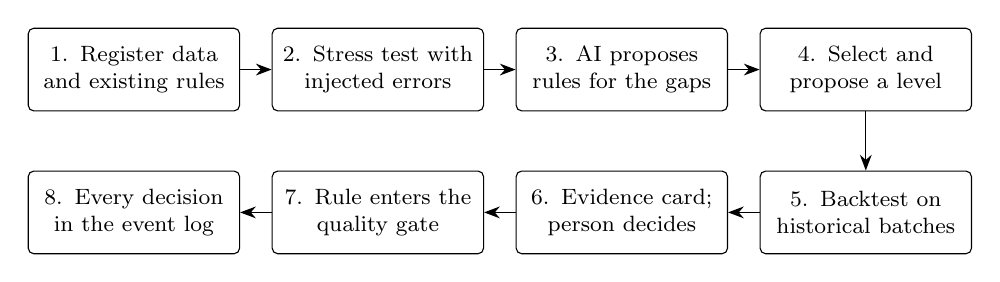
\begin{tikzpicture}[
  box/.style={draw, rounded corners=2pt, align=center, font=\footnotesize, minimum height=1.05cm, text width=2.45cm},
  arr/.style={-{Stealth[length=2mm]}}]
\node[box] (a) {1. Register data\\ and existing rules};
\node[box, right=0.4cm of a] (b) {2. Stress test with\\ injected errors};
\node[box, right=0.4cm of b] (c) {3. AI proposes\\ rules for the gaps};
\node[box, right=0.4cm of c] (d) {4. Select and\\ propose a level};
\node[box, below=0.75cm of d] (e) {5. Backtest on\\ historical batches};
\node[box, left=0.4cm of e] (f) {6. Evidence card;\\ person decides};
\node[box, left=0.4cm of f] (g) {7. Rule enters the\\ quality gate};
\node[box, left=0.4cm of g] (h) {8. Every decision\\ in the event log};
\draw[arr] (a) -- (b); \draw[arr] (b) -- (c); \draw[arr] (c) -- (d);
\draw[arr] (d) -- (e); \draw[arr] (e) -- (f); \draw[arr] (f) -- (g); \draw[arr] (g) -- (h);
\end{tikzpicture}
\caption{The workbench. It never adopts a rule by itself and never changes data.}
\label{fig:tool}
\end{figure}

The workbench keeps a register of all rules, expert and AI-written, with their version, the date from which each rule was available, its level and every decision about it. For each proposed rule it produces an evidence card: which injected errors the rule catches that existing rules miss, how many alerts it raises per week in the backtest, how stable it is across periods and across regenerations, and the level it is proposed for. A person decides, and the decision is stored in an append-only event log. We do not rely on the version history of the data tables for this, because old versions are removed after a retention period, by default seven days \cite{vacuum}.

We demonstrate the quality gate in a small pipeline built with Apache Spark and Delta Lake, two open-source technologies that are widely used in data platforms \cite{spark,deltalake}. New SEC reports land in a staging area, Arelle runs the expert rules, the approved AI rules run next, and each batch is then published, published with warnings, or held in quarantine according to the rule levels. The same workbench can backtest hand-written rules, so its use is not limited to AI. We evaluate the artefact in three ways: all experiments run through it with one command per experiment; it is delivered with tests, documentation and an open-source licence; and, if time and ethics approval allow, three to five data professionals review evidence cards while we record their decisions and the time they need.

\section{Expected contributions}

Several parts of this work exist already and are not claimed: LLMs that write data-quality rules \cite{ledqer,audq,akella,siyam,schneider}, comparison with a small expert reference \cite{schneider,alexander}, selection of generated checks under a false-alarm limit \cite{spade,autovalidate}, validation of recurring pipelines over time \cite{redyuk,avh}, checked write paths in lakehouses \cite{tagliabue}, and LLMs as judges of financial reports \cite{finauditing,secfintables}. Systems that generate and store data-quality rules with LLMs are also patented \cite{patent}.

The expected contributions are:
\begin{enumerate}
\item an evaluation of AI-written rules against large, independent expert rule sets using official answer keys, with a contamination analysis and a comparison between judging a rule by reading and judging it by running it;
\item a selection method that keeps only AI-written rules that add to the existing expert rules within a review budget, compared with four alternatives, and evidence on whether such selection can assign a safe level (block, warn or monitor);
\item a backtest of the selected rules on historical financial reports in filing order, with verified real errors as reference, and a public set of verified errors (D5);
\item an open-source workbench and pipeline that test new data checks on historical data before use.
\end{enumerate}
This field changes quickly, so the literature will be checked again every month and the claims adjusted where needed.

\section{Planning and risks}

\begin{table}[htbp]
\centering
\small
\begin{tabularx}{\textwidth}{@{}p{1.5cm}L@{}}
\toprule
Month & Work \\
\midrule
1 & Protocol; ethics request; cluster access; labelling guide; rule register and backtest engine for D1 \\
2 & RQ1 on D1, including the contamination analysis; GLEIF test records \\
3 & RQ2 on D1; start labelling D5. End of month: decision point (see below) \\
4 & RQ1 and RQ2 on D2 and D3; Spark and Delta Lake pipeline with the quality gate \\
5 & RQ3 backtests; D5 and the reviewed alert sample completed \\
6 & RQ3 analysis; evidence cards and approval screen; optional review by professionals \\
7 & Robustness checks; demonstration to Avanade and Rabobank \\
8--9 & Writing; buffer \\
\bottomrule
\end{tabularx}
\caption{Nine-month plan.}
\label{tab:plan}
\end{table}

At the end of month 3 we check progress. If the core (D1 with RQ1 to RQ3, and D5) is on schedule, the extensions go ahead; otherwise we cut in this order: D4, then D3, then the depth of D2, then the number of models.

\begin{table}[htbp]
\centering
\small
\begin{tabularx}{\textwidth}{@{}LL@{}}
\toprule
Risk & Response \\
\midrule
AI rules add little, even with larger models & The thesis is a measurement; a clear negative answer with its causes is a valid result. \\
Few verified real errors are visible in the original report & Weight the D5 sample towards correction types that are more often data errors; report RQ3 with confidence intervals. \\
Never-corrected reports are treated as correct & Count their alerts as an upper bound only; estimate false alarms from the reviewed sample. \\
Hidden use of future information in the backtest & Record availability dates for every rule and model; run the time-bound form only after the model's release. \\
Building the pipeline crowds out the research & Keep the pipeline small (SEC only); the scientific results come from RQ1 to RQ3. \\
Ethics approval or professionals' time & Request approval in month one; a fellow student can act as second labeller. \\
\bottomrule
\end{tabularx}
\caption{Main risks.}
\label{tab:risks}
\end{table}

\section{Value for Avanade and Rabobank}

The thesis gives a data team three things it can use without sharing any data: evidence on what to expect from AI-written rules, a procedure to decide which rules to adopt and at which level, and a tool that backtests a new rule on the team's own history before it goes live. Because the tool runs locally with an open-weight model, it can be tried on internal data under the bank's own approval process.

\begin{thebibliography}{99}
\footnotesize
\setlength{\itemsep}{0pt}
\setlength{\parskip}{0pt}

\bibitem{tran} L. Tran, correspondence with the author, 4 September 2026 (unpublished; observations specific to his working context).

\bibitem{bcbs239} Basel Committee on Banking Supervision, ``Principles for effective risk data aggregation and risk reporting,'' Bank for International Settlements, January 2013.

\bibitem{ecbrdarr} European Central Bank, ``Guide on effective risk data aggregation and risk reporting,'' May 2024.

\bibitem{rehberger} T. Rehberger, T. H\"utter, L. Ehrlinger, and W. W\"o{\ss}, ``Evaluating Data Quality Tools: Measurement Capabilities and LLM Integration,'' arXiv:2604.09163, 2026.

\bibitem{ouyang} S. Ouyang, J. M. Zhang, M. Harman, and M. Wang, ``An Empirical Study of the Non-Determinism of ChatGPT in Code Generation,'' ACM Transactions on Software Engineering and Methodology, vol. 34, no. 2, 2025. doi:10.1145/3697010.

\bibitem{martin} A. Martin, E. C. de Almeida, O. Romero, and A. Queralt, ``How and Why False Denial Constraints are Discovered,'' Proceedings of the VLDB Endowment, vol. 18, no. 10, pp. 3477--3489, 2025. doi:10.14778/3748191.3748209.

\bibitem{abedjan} Z. Abedjan, X. Chu, D. Deng, R. C. Fernandez, I. F. Ilyas, M. Ouzzani, P. Papotti, and M. Stonebraker, ``Detecting Data Errors: Where are we and what needs to be done?,'' Proceedings of the VLDB Endowment, vol. 9, no. 12, pp. 993--1004, 2016. doi:10.14778/2994509.2994518.

\bibitem{rein} M. Abdelaal, C. Hammacher, and H. Schoening, ``REIN: A Comprehensive Benchmark Framework for Data Cleaning Methods in ML Pipelines,'' Proceedings of EDBT, pp. 499--511, 2023.

\bibitem{deequ} S. Schelter, D. Lange, P. Schmidt, M. Celikel, F. Biessmann, and A. Grafberger, ``Automating Large-Scale Data Quality Verification,'' Proceedings of the VLDB Endowment, vol. 11, no. 12, pp. 1781--1794, 2018. doi:10.14778/3229863.3229867.

\bibitem{alexander} R. Alexander, L. Katz, C. Moore, M. W.-C. Wong, and Z. Schwartz, ``Evaluating the Decency and Consistency of Data Validation Tests Generated by LLMs,'' arXiv:2310.01402, 2023.

\bibitem{ledqer} A.-C. Glock, T. H\"utter, J. F\"urnkranz, W. W\"o{\ss}, A. Dominka-Kiss, and L. Ehrlinger, ``Data Quality Rule Generation with LLMs,'' arXiv:2609.06053, 2026.

\bibitem{audq} J. Biggiogera, N. Colombo, K. Saxena, B. Sarmah, and S. Pasquali, ``AuDQ: Auditable Data Quality through Agentic Rule Discovery,'' arXiv:2610.26031, 2026.

\bibitem{akella} A. Akella, A. Kaul, K. Narayanam, and S. Mehta, ``Quality Assessment of Tabular Data using Large Language Models and Code Generation,'' Proceedings of EMNLP 2025: Industry Track, pp. 2713--2748, 2025. doi:10.18653/v1/2025.emnlp-industry.183.

\bibitem{fadlallah} Fadlallah et al., ``An Agentic Retrieval Framework for Autonomous Context-Aware Data Quality Assessment,'' arXiv:2606.13692, 2026.

\bibitem{siyam} S. Siyam, ``Evaluating the Effectiveness of LLMs and Prompting Techniques in Generating Data Quality Rules,'' MSc thesis, University of Jyv\"askyl\"a, 2025.

\bibitem{schneider} A. Schneider, ``Template-Guided Rule Generation and Evaluation for Data Quality,'' MSc thesis, TU Wien, 2025.

\bibitem{spade} S. Shankar, H. Li, P. Asawa, M. Hulsebos, Y. Lin, J. D. Zamfirescu-Pereira, H. Chase, W. Fu-Hinthorn, A. G. Parameswaran, and E. Wu, ``SPADE: Synthesizing Data Quality Assertions for Large Language Model Pipelines,'' arXiv:2401.03038, 2024.

\bibitem{autovalidate} J. Song and Y. He, ``Auto-Validate: Unsupervised Data Validation Using Data-Domain Patterns Inferred from Data Lakes,'' Proceedings of SIGMOD, 2021.

\bibitem{redyuk} S. Redyuk, Z. Kaoudi, V. Markl, and S. Schelter, ``Automating Data Quality Validation for Dynamic Data Ingestion,'' Proceedings of EDBT, 2021.

\bibitem{avh} D. Tu, Y. He, W. Cui, S. Ge, et al., ``Auto-Validate by-History: Auto-Program Data Quality Constraints to Validate Recurring Data Pipelines,'' Proceedings of KDD, 2023. arXiv:2306.02421.

\bibitem{lakehouse} M. Armbrust, A. Ghodsi, R. Xin, and M. Zaharia, ``Lakehouse: A New Generation of Open Platforms that Unify Data Warehousing and Advanced Analytics,'' Proceedings of CIDR, 2021.

\bibitem{spark} M. Zaharia et al., ``Apache Spark: A Unified Engine for Big Data Processing,'' Communications of the ACM, vol. 59, no. 11, pp. 56--65, 2016.

\bibitem{deltalake} M. Armbrust et al., ``Delta Lake: High-Performance ACID Table Storage over Cloud Object Stores,'' Proceedings of the VLDB Endowment, vol. 13, no. 12, pp. 3411--3424, 2020.

\bibitem{tagliabue} J. Tagliabue and C. Greco, ``Safe, Untrusted, `Proof-Carrying' AI Agents: toward the agentic lakehouse,'' IEEE Big Data Workshop on Secure and Safe AI Agents for Big Data Infrastructures, 2025. arXiv:2510.09567.

\bibitem{eltbench} T. Jin, Y. Zhu, and D. Kang, ``ELT-Bench: An End-to-End Benchmark for Evaluating AI Agents on ELT Pipelines,'' Proceedings of the VLDB Endowment, vol. 19, 2025. arXiv:2504.04808.

\bibitem{bcbs1996} Basel Committee on Banking Supervision, ``Supervisory framework for the use of `backtesting' in conjunction with the internal models approach to market risk capital requirements,'' January 1996.

\bibitem{joel} S. Joel, J. J. Wu, and F. H. Fard, ``A Survey on LLM-based Code Generation for Low-Resource and Domain-Specific Programming Languages,'' ACM Transactions on Software Engineering and Methodology (accepted), arXiv:2410.03981.

\bibitem{livecodebench} N. Jain, K. Han, A. Gu, W.-D. Li, F. Yan, T. Zhang, S. Wang, A. Solar-Lezama, K. Sen, and I. Stoica, ``LiveCodeBench: Holistic and Contamination Free Evaluation of Large Language Models for Code,'' Proceedings of ICLR, 2025.

\bibitem{olmo2} Team OLMo, ``2 OLMo 2 Furious,'' arXiv:2501.00656, 2024.

\bibitem{olmotrace} J. Liu et al., ``OLMoTrace: Tracing Language Model Outputs Back to Trillions of Training Tokens,'' Proceedings of ACL 2025: System Demonstrations. arXiv:2504.07096.

\bibitem{fintagging} Y. Wang, L. Qian, X. Peng, et al., ``FinTagging: Benchmarking LLMs for Extracting and Structuring Financial Information,'' arXiv:2505.20650, 2025.

\bibitem{finauditing} Y. Wang, K. Wang, S. Yang, J. Patel, et al., ``FinAuditing: A Financial Taxonomy-Structured Multi-Document Benchmark for Evaluating LLMs,'' arXiv:2510.08886, 2025.

\bibitem{secfintables} S. Ke, Q. Wu, H. Li, and L. Cao, ``SEC-FinTables: Evaluating Large Language Models for Detecting Logical Inconsistencies on Tabular Data,'' Findings of ACL 2026, pp. 15587--15607, 2026.

\bibitem{debreceny} R. Debreceny, S. Farewell, M. Piechocki, C. Felden, and A. Gr\"aning, ``Does it add up? Early evidence on the data quality of XBRL filings to the SEC,'' Journal of Accounting and Public Policy, vol. 29, no. 3, pp. 296--306, 2010.

\bibitem{brown} N. C. Brown, R. M. Crowley, and W. B. Elliott, ``What Are You Saying? Using Topic to Detect Financial Misreporting,'' Journal of Accounting Research, vol. 58, no. 1, pp. 237--291, 2020.

\bibitem{pilotreport} T. Oosterbaan, ``Data-quality controls with and without AI: what two pilot studies showed,'' project repository \texttt{masterthesis\_direction3\_pilot}, October 2026.

\bibitem{feasibility} T. Oosterbaan, ``Backtest feasibility check,'' project repository \texttt{masterthesis\_direction3\_pilot}, file \texttt{docs/backtest\_feasibility.md}, 1 November 2026.

\bibitem{cdc} S. J\"ager and F. Biessmann, ``From Data Imputation to Data Cleaning: Automated Cleaning of Tabular Data Improves Downstream Predictive Performance,'' Proceedings of AISTATS, PMLR 238, pp. 3394--3402, 2024.

\bibitem{raha} M. Mahdavi, Z. Abedjan, R. C. Fernandez, S. Madden, M. Ouzzani, M. Stonebraker, and N. Tang, ``Raha: A Configuration-Free Error Detection System,'' Proceedings of SIGMOD, pp. 865--882, 2019.

\bibitem{taberr} P. Jung, S. J\"ager, N. Chandler, and F. Biessmann, ``Towards Realistic Error Models for Tabular Data,'' ACM Journal of Data and Information Quality, vol. 17, no. 4, article 28, 2025.

\bibitem{dqc} XBRL US Data Quality Committee, ``DQC rules (dqc\_us\_rules),'' rules, documentation and test suite, version 31. \url{https://github.com/DataQualityCommittee/dqc_us_rules}

\bibitem{fsds} U.S. Securities and Exchange Commission, ``Financial Statement Data Sets,'' quarters 2023q1 to 2025q2. \url{https://www.sec.gov/data-research/sec-markets-data/financial-statement-data-sets}

\bibitem{esefdqr} XBRL International, ``ESEF Data Quality Rules.'' \url{https://esef-dqr.xbrl.org}

\bibitem{dqrconf} XBRL International, ``ESEF DQR Conformance Suite.'' \url{https://gitlab.xbrl.org/xii/dqr-conformance}

\bibitem{hmda} Federal Financial Institutions Examination Council and Consumer Financial Protection Bureau, ``Filing Instructions Guide for HMDA data collected in 2025.'' \url{https://ffiec.cfpb.gov/documentation/fig/2025/overview}

\bibitem{hmdaplatform} Consumer Financial Protection Bureau, ``HMDA Platform,'' open-source filing and validation software. \url{https://github.com/cfpb/hmda-platform}

\bibitem{gleif} Global Legal Entity Identifier Foundation, ``Data Quality Rule Setting,'' version 3.5. \url{https://www.gleif.org/en/lei-data/gleif-data-quality-management}

\bibitem{arelle} Arelle, open-source XBRL platform. \url{https://arelle.org}

\bibitem{cohen} J. Cohen, ``A Coefficient of Agreement for Nominal Scales,'' Educational and Psychological Measurement, vol. 20, no. 1, pp. 37--46, 1960.

\bibitem{habrok} University of Groningen, ``Hábrók high-performance computing cluster: Apptainer containers.'' \url{https://wiki.hpc.rug.nl/habrok/examples/apptainer}

\bibitem{qwen25coder} B. Hui, J. Yang, Z. Cui, J. Yang, et al., ``Qwen2.5-Coder Technical Report,'' arXiv:2409.12186, 2024.

\bibitem{qwen3} A. Yang, A. Li, B. Yang, B. Zhang, et al., ``Qwen3 Technical Report,'' arXiv:2505.09388, 2025.

\bibitem{gptoss} OpenAI, ``gpt-oss-120b \& gpt-oss-20b Model Card,'' arXiv:2508.10925, 2025.

\bibitem{vacuum} Databricks, ``VACUUM,'' SQL language reference: the default retention threshold for removed data files is seven days. \url{https://docs.databricks.com/aws/sql/language-manual/delta-vacuum}

\bibitem{patent} ``Systems and methods for automatically ensuring data quality using LLMs,'' U.S. Patent 12,632,447.

\end{thebibliography}

\end{document}
